\chapter{Current Work}
\label{currentwork}

The initial aim of this research is to construct a process calculus which
combines the notions of discrete time and mobility.  Earlier work
during an undergraduate project focused on developing a semantics for
the Cashews\footnote{Cashews is a language for web service
  composition, initially based on OWL-S.}\cite{cashews-sem} language,
using the CaSE process calculus (see section \ref{tplext}) and later,
a conservative extension to it called Cashew-Nuts.  It became clear
during this project that it would be interesting to further extend CaSE
with a notion of mobility, and this led to the development of the
calculus of \emph{Typed Nomadic Time} (TNT) discussed here.

\section{The Calculus of Synchronous \\ Encapsulation (CaSE)}
\label{case}

The syntax for CaSE, given in \cite{norton05alg}, is as follows:
\begin{equation}
  \begin{aligned}
    \expr, \exprb\ ::=\ &
    \nil  \;\,|\,\; 
    \Delta \;\,|\,\; 
    \Delta_{\sigma} \;\,|\,\; 
    \alpha . \expr  \;\,|\,\;
    \expr + \exprb \;\,|\,\; 
   \expr \mathrel{\!|\!} \exprb \mid
    \timeout{\expr}{\sigma}{\exprb} \;\,|\,\; \\
    & \stimeout{\expr}{\sigma}{\exprb} \;\,|\,\; 
    \mu X . \expr \;\,|\,\; 
    X \;\,|\,\; 
    \expr \setminus a \;\,|\,\; 
    \expr / \sigma
  \end{aligned}
\end{equation}
where $\expr$ and $\exprb$ define possible process terms. We assume a
countable set of actions, $\actions = \names \cup \conames \cup
\{\tau\}$, ranged over by $\alpha$, where the elements of $\names$ are
drawn from an infinite set of \emph{names}, and $\conames$ is the
corresponding set of \emph{co-names}, $\{\overline{a} \mid a \in
\names\}$. $\timers$ is a countably infinite set of \emph{clocks} over
which $\sigma$ ranges. $X$ ranges over a countably infinite set of variables, which are used to bind process
behaviour in recursive process definitions. $\nil$, $\alpha . \expr$,
$\expr + \exprb$, $\expr \mathrel{\!|\!} \exprb$, $\mu X
. \expr$, $X$ and $\expr \setminus a$ retain their behaviour defined in
CCS, but now exhibit additional actions due to the presence of clocks.

There are now transitions for the $\nil$ process, as, while the
process has no explicit behaviour, it can idle over the ticks of the
clocks.  This also applies to actions in general:

\begin{equation}
a.0 \derives{\sigma} a.0
\end{equation}

\noindent assuming a clock context containing just the one clock,
$\sigma$. Similarly, non-deterministic choice and parallel composition
exist through time, so both sides can evolve due to a clock tick,
while the operator remains in place.  This gives the following
possible derivations for $a.0\;|\;b.0$ (where $b \ne \overline{a}$):

\begin{enumerate}
\item $a.0\ |\ b.0 \derives{a} 0\ |\ b.0$
\item $a.0\ |\ b.0 \derives{b} a.0\ |\ 0$
\item $a.0 |\ b.0 \derives{\sigma} a.0\ |\ b.0$
\end{enumerate}

\noindent with the same clock context as above.  The third derivation
is duplicated for each available clock that can tick over both sides
of the composition.  In cases where both sides may synchronize,
causing a $\tau$ transition, this takes precedence over the clock
transitions, due to \emph{maximal progress} (see \ref{timing}) and the
original set of derivations for parallel composition (see \ref{ccs})
are available instead.

The changes to non-deterministic choice are simpler, as the operator itself
does not generate silent actions.  So, if both sides allow the clock to tick,
then the following derivations will occur:

\begin{enumerate}
\item $a.0\ +\ b.0 \derives{a} 0$
\item $a.0\ +\ b.0 \derives{b} 0$
\item $a.0\ +\ b.0 \derives{\sigma} a.0\ +\ b.0$
\end{enumerate}

\noindent again with the single clock, $\sigma$, as the context.

\subsection{Timeouts}

Moving on to the new operators, CaSE, as presented in
\cite{norton05alg}, includes two variants of the timeout operator,
first seen in TPL.  Recall from \ref{timing} that the operator
essentially allows a decision to be made, based on the presence of a
clock tick.  In the general scenario,

\begin{equation}
\timeout{E}{\sigma}{F}
\end{equation}

\noindent $F$ will act if $E$ fails to, prior to a clock tick.  If $E$
can perform a $\tau$ action, then this will prevent the clock tick and
$E$ will evolve. Both operators in CaSE maintain this core behaviour,
which is central to the concept of global synchronization explained
earlier.

The difference between the two operators in CaSE lies in their
behaviour with regard to other clocks.  With the fragile timeout,
$\timeout{E}{\sigma}{F}$, any possible transition on $E$ will cause the
removal of the timeout.  So, with $\timeout{a.0}{\sigma}{b.0}$ and a clock
context of $\sigma$ and $\rho$, the following derivations can occur:

\begin{enumerate}
\item $\timeout{a.0}{\sigma}{b.0} \derives{a} 0$
\item $\timeout{a.0}{\sigma}{b.0} \derives{\sigma} b.0$
\item $\timeout{a.0}{\sigma}{b.0} \derives{\rho} a.0$
\end{enumerate}

\noindent where both the $a$ and the $\rho$ transition leave only the
left-hand side of the timeout.

The stable timeout differs by continuing to exist through time until
some action occurs.  While it exhibits the same behaviour in response
to actions or the tick of the specified clock, the ticks of other
clocks only cause the left-hand side to evolve; the timeout itself is
retained.  Thus, $\stimeout{a.0}{\sigma}{b.0}$ gives a different set
of derivations:

\begin{enumerate}
\item $\stimeout{a.0}{\sigma}{b.0} \derives{a} 0$
\item $\stimeout{a.0}{\sigma}{b.0} \derives{\sigma} b.0$
\item $\stimeout{a.0}{\sigma}{b.0} \derives{\rho} \stimeout{a.0}{\sigma}{b.0}$
\end{enumerate}

\noindent where the $\rho$ transition no longer causes the dissolution
of the timeout.

\subsection{Clock Stopping and Insistency}
\label{clockcontrol}

The remaining operators further control the behaviour of the clocks.
$\Delta$ prevents all clocks from ticking, while $\Delta_{\sigma}$
prevents only the ticks of the specified clock, $\sigma$.  $\Delta$ is
similar to the CCS version of $\nil$, as it has no possible
transitions.  $\Delta_{\sigma}$ exhibits transitions for all other
clocks within the current context.  So, for a context containing both
$\sigma$ and $\rho$, $\Delta_{\sigma}$ has a single transition,

\begin{equation}
  \Delta_{\sigma} \derives{\rho} \Delta_{\sigma}
\end{equation}

\noindent which is replicated for any other clocks in the context,
which are not equal to $\sigma$.

The stopping of clocks is used to provide \emph{insistency}.  Normally,
a process $a.P$ has two possible derivations:

\begin{enumerate}
  \item $a.P \derives{a} P$
  \item $a.P \derives{\sigma} P$
\end{enumerate}

\noindent with a clock context containing only $\sigma$.  To ensure
that the first of these two derivations occurs, or, in other words, to
\emph{insist} that $a$ is performed before the next tick of the clock,
$\sigma$, $\Delta$ is used.  The semantics for an insistent prefix,
$\underline{\alpha}.P$, may be given as:

\begin{equation}
\seml \underline{\alpha}.P \semr \eqdef \alpha.P + \Delta 
\end{equation}

\noindent where the presence of $\Delta$ prevents a $\sigma$
transition from occurring on the right-hand side of the choice, and
thus for the choice as a whole (as both sides must move through time
simultaneously).  This leaves only one available action,
$\derives{a}$, as required.  Clearly, insistency relative only to one
particular clock may also be defined in a similar manner, using
$\Delta_{\sigma}$ instead.

\begin{equation}
\seml \underline{\alpha}_{\sigma}.P \semr \eqdef \alpha.P + \Delta_{\sigma} 
\end{equation}

While on the subject of derived syntax, it is also possible to define
a clock prefix, akin to the existing action prefix:

\begin{equation}
\seml \sigma.P \semr \eqdef \stimeout{\nil}{\sigma}{P}
\end{equation}

\noindent where the stable timeout ensures that the $\sigma.P$ will be
retained until $\sigma$ ticks, despite the ticks of other clocks.  As
the only transitions for $\nil$ are clock ticks, only a tick from
$\sigma$ will cause the process to evolve and become $P$.

The two notions of a clock prefix and insistency can then be combined
to give an insistent clock prefix:

\begin{equation}
\seml \underline{\sigma}.P \semr \eqdef \stimeout{\Delta}{\sigma}{P}
\end{equation}

\noindent which differs from a standard clock prefix by only ever
allowing the one transition, $\underline{\sigma}.P \derives{\sigma}
P$, whereas $\sigma.P$ allows an arbitrary number of transitions from
other clocks before this occurs.

\subsection{Encapsulation}

Clock hiding is used to provide scoping for the ticks of a
clock.  Take the following situation,

\begin{equation}
\label{clockhidingex}
  (P / \sigma)\;|\;Q
\end{equation}

\noindent where $/ \sigma$ hides the clock, $\sigma$, so that its
ticks may only be seen by $P$.  $Q$ instead sees a silent action each
time $\sigma$ ticks.  Such clock hiding is central to the
encapsulation of components present in CaSE.  When coupled with
restriction, components can be made to emit only silent actions from
the perspective of external processes.

\section{Localising the Calculus}

\emph{Localisation}, discussed in detail in \ref{migration}, effectively
adds another level of grouping to the calculus.  A set of composed
processes may be contained within one \emph{locality}, a notion which is
often used in the modelling of \emph{distribution}.  This idea, which
can be taken to its logical conclusion by forming a hierarchy of such
localities, has echoes of the notion of \emph{clock hiding} within CaSE,
as just described.

Thus, the first step in the evolution towards TNT is to combine these
two hierarchical concepts by effectively localising CaSE.  The notion of
components and encapsulation is explicitly realised by an
\emph{environ}, which also handles the hiding of clocks.  As a result,
the clock hiding operator from CaSE disappears, being replaced by a new
operator which allows the creation of localities.  The bounds of the
environ define both a new group and the scope of the clock hiding.  The
syntax for localised CaSE is thus:
\begin{equation}
  \begin{aligned}
    \expr, \exprb\ ::=\ &
    \nil  \;\,|\,\; 
    \Delta \;\,|\,\; 
    \Delta_{\sigma} \;\,|\,\; 
    \alpha . \expr  \;\,|\,\;
    \expr + \exprb \;\,|\,\; 
    (\expr\;|\;\exprb)\;\,|\,\; 
    \timeout{\expr}{\sigma}{\exprb} \;\,|\,\; \\
    & \stimeout{\expr}{\sigma}{\exprb} \;\,|\,\; 
    \mu X . \expr \;\,|\,\; 
    X \;\,|\,\; 
    \expr \setminus a \;\,|\,\; 
    \lclocv{m}{\expr}{\vec{\sigma}}
  \end{aligned}
\end{equation}
where $m$ represents an arbitrary locality name\footnote{Note
that although names are added to the localities here, this is not really
necessary at this stage; they provide nothing more than a way to refer
to localities in talking about a system.  However, they are necessary
for providing migration as discussed in \ref{migration}}.  In
particular, $m$ may be equal to the empty string, $\epsilon$, thus
facilitating the use of anonymous localities.  This allows the semantics
of CaSE's clock hiding to be encoded:

\begin{equation}
\seml E / \sigma \semr \eqdef \lcloc{}{E}{\sigma}
\end{equation}

\noindent thus making localised CaSE a conservative extension.  The
environs form a forest structure, due to the ability to nest
environs to an arbitrary depth and the possibility of multiple
environs occurring at the top level.

Recall the example of clock hiding above (\ref{clockhidingex}).  This
becomes:
\begin{equation}
  \lcloc{}{P}{\sigma}\;|\;Q
\end{equation}
in localised CaSE, or:
\begin{equation}
  \lcloc{m}{P}{\sigma}\;|\;Q
\end{equation}
if an arbitrary name, $m$, is assigned to the environ.  Just
as with the clock hiding operator, the clock $\sigma$ is hidden outside
the environ, $m$, causing its ticks to be visible only to $P$.  

With this extension the set of visible clocks for a particular environ
may be obtained by taking the union of its set of clocks and the sets of
the parent environs.  For example, consider the more complex scenario:
\begin{equation}
\lcloc{n}{E\;|\;\lcloc{m}{F\;|\;\lcloc{k}{G}{\sigma}}{\rho}}{\gamma}
\end{equation}
where the top-level environ, $n$, contains a process $E$ and
a further sub-environ, $m$.  Likewise, $m$ contains both a process,
$F$, and the sub-environ, $k$.  Finally, $k$ contains just the single
process, $G$.  The set of clocks for the environ $k$ is $\{\sigma\}$
and its parents are $m$ (with the set $\{\rho\}$) and $n$ (with
$\{\gamma\}$).  Thus, the set of visible clocks for $k$ is $\{\sigma\}
\cup \{\rho\} \cup \{\gamma\}$ or simply $\{\sigma, \rho, \gamma\}$,
which means that $G$, located in $k$, can see the ticks of all three
clocks.

$F$, by comparison, can only see the ticks of the clocks, $\rho$ and
$\gamma$, as $\sigma$ is hidden outside $k$.  $E$, in the top-level
environ, $n$, can only observe silent actions resulting from the two
hidden clocks, $\rho$ and $\sigma$, but can see the ticks of $\gamma$.
Taking this further, it is clear that the clock context, the set of
clocks within the system, can be derived as the union of the sets of
clocks associated with each environ ($\{\sigma, \rho, \gamma\}$ in
this case).

\section{Adding Mobility}
\label{addingmob}

Localised CaSE makes the notion of components and encapsulation clearer
than in the original calculus, by allowing them to be given explicit
names.  However, it doesn't provide a great deal of extra
functionality\footnote{Although the semantics could be adapted so as to
use the localities for bisimulation, as in \ref{migration}.}.  The most
natural progression from this stage is to add mobility.  For this, the
primitives of the ambient calculus are adopted, as they provide a very
natural and simplistic formalism, which builds on the component-oriented
nature of the calculus, now explicitly realised by environs.  This is
shown in more detail in \ref{locmob}.

In addition, TNT allows the movement of individual processes.  In the
ambient calculus, only ambients can move, which restricts the
separability of processes.  For a given group of processes, the
size of the group may only change by:

\begin{enumerate}
\item One of the processes becoming $\nil$.  Both TNT and the ambient
      calculus include a structural congruence law,
\begin{equation}
E\;|\;\nil \equiv E
\end{equation}
      which allows such processes to be removed.
\item The process splitting into two or more processes via parallel
      composition.  For example, $\ambin{m}.(E | F)$ enters the ambient, $m$,
      and then splits into two separate processes, $E$ and $F$.
\item Another process \emph{open}ing the ambient, causing the set of
      processes to merge with those in the parent.
\end{enumerate}

What the ambient calculus doesn't allow is for a selected process or
group of processes to be moved from one ambient to another.  That
process or group must be in its own ambient for this to happen.

Take the example process, 
\begin{equation}
m[E\;|\;F\;|\;G]\;|\;n[\nil]\;|\;H
\end{equation}
where $E$, $F$, $G$ and $H$ are all processes and $m$ and $n$
are ambients.  The topology of this process may change in several ways, as
outlined above. Any of the four processes might evolve to $\nil$, or fork
into two or more processes.  In addition, $E$, $F$ or $G$ may emit an
$\ambin{n}$ capability, causing the ambient $m$ to move inside $n$.
Similarly, $H$ may perform an $\ambopen{m}$, causing $m$ to be removed and
the top-level to include all four processes.

So, several events may occur but there are also some that are intuitive,
but difficult to achieve.  For instance, all three processes in $m$ must
move as a unit, whether this is to the top-level due to an $open$
capability or as a result of $m$ moving in to $n$.  Moving one process,
$E$ for example, requires the interaction of both $E$ itself and another
process at the final destination.

To move $E$ to the top level on its own requires converting it to the
form,
\begin{equation}
Emov \eqdef z[\ambout{m}.E]
\end{equation}
where $z$ is a new name, which doesn't occur free in either
$E$, $F$, $G$ or $H$.  The effect is clearer when this is placed in
context,
\begin{equation}
m[z[\ambout{m}.E]\;|\;F\;|\;G]\;|\;n[\nil]\;|\;H
\end{equation}
where it can be clearly seen that the new capability prefixed
on $E$ will cause the new surrounding ambient, $z$, to move outside of
$m$.  To actually have $E$ at the top-level, and not $E$ nested in an
ambient, requires the presence of a top-level process to open the $z$
ambient.  This results in something along the lines of:
\begin{equation}
m[z[\ambout{m}.E]\;|\;F\;|\;G]\;|\;n[\nil]\;|\;H\;|\;\ambopen{z}.\nil
\end{equation}
to truly encode the movement of $E$ alone.  Moving just $E$
into $n$ is even more convoluted:
\begin{equation}
m[z[\ambout{m}.\ambin{n}.E]\;|\;F\;|\;G]\;|\;n[\ambopen{z}.\nil]\;|\;H
\end{equation}
and neither are particularly natural.  TNT instead provides
this functionality as a base part of the syntax, which will be explored
in \ref{procmob}.  

Finally, it should be noted that the scope of an action is implicitly
restricted to the bounds of an environ within TNT.  For instance, in the
following process:
\begin{equation}
a.P \pc \lcloc{m}{\overline{a}.Q}{\sigma}
\end{equation}
synchronization between the two processes is not permitted as
they lie on either side of a environ boundary.  This is not an issue,
as the presence of mobility allows processes to move into a situation
where the co-action is in scope.  In addition, TNT (at present) does not
incorporate the scoping of environ names.

\subsection{Location Mobility}
\label{locmob}

To add an ambient calculus style of mobility, the existing syntax of
localised CaSE is extended with a mobility prefix, $\ambop . \expr$,
to give:
\begin{equation}
  \begin{aligned}
    \expr, \exprb \mathrel{::=} &
    \nil  \;\,|\,\; 
    \Delta \;\,|\,\; 
    \Delta_{\sigma} \;\,|\,\; 
    \alpha . \expr  \;\,|\,\;
    \expr + \exprb \;\,|\,\; 
    (\expr\;|\;\exprb)\;\,|\,\; 
    \timeout{\expr}{\sigma}{\exprb} \;\,|\,\; \\
    & \stimeout{\expr}{\sigma}{\exprb} \;\,|\,\; 
    \mu X . \expr \;\,|\,\; 
    X \;\,|\,\; 
    \expr \setminus a \;\,|\,\; 
    \lcloc{m}{\expr}{\vec{\sigma}} \;\,|\,\;
    \ambop . \expr
  \end{aligned}
\end{equation}
where $\ambop$ is further defined as:
\begin{equation}
   \ambop \mathrel{::=} \tntin{m} \mid \tntout{m} \mid \tntopen{m} 
\end{equation}
with $m$ again representing the name of an environ.  The behaviour of
these primitives is identical to the behaviour of their equivalents in
the ambient calculus ($\tntin{m}$ being $\ambin{m}$, $\tntout{m}$ being
$\ambout{m}$ and $\tntopen{m}$ being $\ambopen{m}$)\footnote{The mnemonics
$\tntin{m}$, $\tntout{m}$ and $\tntopen{m}$ are used to prevent
confusion with the names of actions.}, so just a short recap of section
\ref{ambientcalculus} is given here, using the syntax above.  Note that
the syntactic abbreviation, $\lncloc{m}{E}$, is used to represent
$\lcloc{m}{E}{}$.

When a process emits an $\tntin{m}$ capability, the surrounding environ
may move into a sibling environ with the name, $m$.  Given the context,
\begin{equation}
\lncloc{m}{E}\;|\;\lncloc{n}{\nil}
\end{equation}
$E$ may be defined as
\begin{equation}
E \eqdef \tntin{n}.E^\prime
\end{equation}
allowing the derivation
\begin{equation}
\lncloc{m}{E}\;|\;\lncloc{n}{\nil} \derives{\tntin{n}} 
\lncloc{n}{\lncloc{m}{E^\prime}\;|\;\nil}
\end{equation}
to occur.  Similarly, defining $E^\prime$ to be
\begin{equation}
E^\prime \eqdef \tntout{n}.E^{\prime\prime}
\end{equation}
allows the converse
\begin{equation}
\lncloc{n}{\lncloc{m}{E^\prime}\;|\;\nil} \derives{\tntout{n}}
\lncloc{m}{E^{\prime\prime}}\;|\;\lncloc{n}{\nil}
\end{equation}
to take place, $\tntout{m}$ allowing the surrounding environ
to move outside a parent environ named $m$.  As noted above, these are
fairly dull, both being identical to the same primitives in the ambient
calculus.  The behaviour of $\tntopen{m}$ is more interesting, due to
its interaction with the environ's clock environment.

Take the example context,
\begin{equation}
\lcloc{m}{E\;|\;\lcloc{n}{F}{\sigma}}{\rho}
\end{equation}
where $E$ is defined as
\begin{equation}
E \eqdef \tntopen{n}.E^\prime
\end{equation}
and thus may cause the environ, $n$, to be destroyed
\begin{equation}
\lcloc{m}{E\;|\;\lcloc{n}{F}{\sigma}}{\rho} \derives{\tntopen{n}}
\lcloc{m}{E'^\prime\;|\;F}{\sigma, \rho}
\end{equation}
and the two clock environments to merge.  As a result, not
only does the context of $F$ change with respect to nearby processes, as
in the ambient calculus, but now $E$ is also affected.  Prior to the
emission of $\tntopen{n}$, $E$ could only see ticks from the clock
$\rho$.  The ticks of $\sigma$ were converted to silent actions by the
environ barrier.  Following the dissolution of the environ, $n$, these
ticks become visible to $E$.  So, the $open$ capability in TNT not only
changes the environ hierarchy, but also the clock context within the
parent locality.

Just as in the ambient calculus, the reduction of capabilities is
subject to the availability of applicable environs, thus allowing for
stalled capabilities (when there are none) and non-determinism (when
there are several). For example, the process
\begin{equation}
\lcloc{m}{\tntopen{n}.E\;|\;\lcloc{n}{F}{\sigma}\;|\;\lcloc{n}{G}{\gamma}}{\rho}
\end{equation}
has two possible derivations

\begin{enumerate}
\item
      $\lcloc{m}{\tntopen{n}.E\;|\;\lcloc{n}{F}{\sigma}\;|\;\lcloc{n}{G}{\gamma}}{\rho}
      \derives{\tntopen{n}} \lcloc{m}{E \pc F \pc
      \lcloc{n}{G}{\gamma}}{\sigma , \rho}$
\item
      $\lcloc{m}{\tntopen{n}.E\;|\;\lcloc{n}{F}{\sigma}\;|\;\lcloc{n}{G}{\gamma}}{\rho}
      \derives{\tntopen{n}} \lcloc{m}{E \pc \lcloc{n}{F}{\rho} \pc G}{\gamma , \rho}$
\end{enumerate}
and, as a result, two different resulting clock contexts.  In
the full calculus, this non-determinism is restricted by the notion of
\emph{bouncers}, introduced in section \ref{bouncers}, which reduce the possibility of \emph{grave interferences} (see \ref{ambvariants}).  

\subsection{Process Mobility}
\label{procmob}

In TNT, the mobility prefix is further extended as follows:

\begin{equation}
   \ambop \mathrel{::=} \tntin{m} \mid \tntout{m} \mid \tntopen{m} 
      \mid \procin{\beta}{m} \mid \procout{\beta}{m}
\end{equation}

\noindent where $\beta \in \mathcal{N}$ and thus refers to an action.
While the location mobility described above is \emph{subjective} (the
process who requests the move does the move), process mobility, in this form,
is \emph{objective}.  The process which emits one of the two new
capabilities synchronizes with a partner process on the given action,
and it is this partner which actually moves.  The partner will be a
process in the same environ, due to the scoping of actions described
above.

Such behaviour is initially difficult to understand, but can be made
clearer with a simple example.  Take the process,
\begin{equation}
\procin{go}{m}.E \pc go.F \pc \lcloc{m}{\nil}{\sigma}
\end{equation}
\noindent where $E$ is emitting the capability $\procin{go}{m}$, but it
is $go.F$ that will actually move,
\begin{equation}
\procin{go}{m}.E \pc go.F \pc \lcloc{m}{\nil}{\sigma} \derives{\procin{go}{m}}
E \pc \lcloc{m}{F \pc \nil}{\sigma}
\end{equation}
with the continuation, $F$, continuing to evolve in the environ $m$.   

Encoding process mobility in this objective form doesn't prevent it from
being used to perform subjective movement.  As processes can fork, a
process that wishes to move can evolve into a situation where it is
composed in parallel with a new process that exhibits the required
capability.  To demonstrate the converse action, $out$, in the scenario
above, $F$ can be defined as
\begin{equation}
F \eqdef leave.F^\prime \pc \procout{leave}{m}
\end{equation}
where the process on the right moves the one on the left outside $m$.
In context, this performs as follows:
\begin{equation}
E \pc \lcloc{m}{leave.F^\prime \pc \procout{leave}{m}.\nil \pc
 \nil}{\sigma} 
\derives{\procout{leave}{m}}
E \pc F^\prime \pc \lcloc{m}{\nil \pc \nil}{\sigma}
\end{equation}
to give a final process which is very similar to the original.

More generally, a subjective process movement may be encoded as
\begin{equation}
\seml \sprocin{m}{E}.F \semr \eqdef z.E \pc \procin{z}{m}.F
\end{equation}
where $e$ is the process that will move in to $m$, $F$ is
the continuation and $z$ is a new name.  The converse is pretty much the same:
\begin{equation}
\seml \sprocout{m}{E}.F \semr \eqdef z.E \pc \procout{z}{m}.F
\end{equation}

\subsection{Bouncers}
\label{bouncers}

This description of TNT is concluded by the addition of the final
element, the \emph{bouncers}.  Named after the staff who
restrict access to a night club\footnote{American usage:
doorman/woman.}, the bouncer is an additional property of an environ
which appears in the top right of the expression.  It has no real
behaviour of its own, but instead performs the job of protecting the
environ, being a process with a limited choice of available
constructs\footnote{This limited choice is only explicitly imposed by
the type system.  There is no restriction in the abstract syntax.}.  The
bouncer provides a structured selection of co-primitives ($\bin$,
$\bout$ and $\bopen$), similar to those in \cite{sangiorgi:mobsafeambients} (see section \ref{ambvariants}) and dictates which mobility transitions may
occur, and when..

The full syntax of TNT may now be given as:
\begin{equation}
  \begin{aligned}
    \expr, \exprb \quad \mathrel{::=} \quad &
      \nil  \mid
      \Omega \mid
      \Delta \mid
      \Delta_{\sigma} \mid
      \alpha . \expr  \mid
      \expr + \exprb \mid
      \expr \mathrel{\!|\!} \exprb \mid
      \timeout{\expr}{\sigma}{\exprb} \mid \\
    & \stimeout{\expr}{\sigma}{\exprb} \mid 
      \mu X . \expr \mid
      X \mid 
      \expr \res{A} \mid
      \locv{m}{\expr}{\exprb}{\vec{\sigma}} \mid
      \ambop . \expr \\
   \ambop \quad \mathrel{::=} \quad & \tntin{m} \mid \tntout{m} \mid \tntopen{m} \mid
      \procin{\beta}{m} \mid \procout{\beta}{m} \mid \bin \mid
      \bout \mid \bopen
   \end{aligned}
   \label{eqn:tnt-syntax}
\end{equation}
with $\Omega$ representing the bouncer with no behaviour (the
equivalent of $\nil$).  For a process or environ to enter another
environ, its bouncer must allow this to occur by providing the
corresponding $\bin$ co-capability.  Likewise, it must provide $\bout$
to allow a process or environ to leave.  With regard to the destruction
of a environ, the environ's bouncer must allow it to be removed by
providing a $\bopen$ co-capability.

Recall the example given in \ref{locmob}.
\begin{equation}
\lncloc{m}{\tntin{n}.E^\prime}\;|\;\lncloc{n}{\nil}
\end{equation}
With the addition of bouncers, this becomes:
\begin{equation}
\nloc{m}{\tntin{n}.E^\prime}{\Omega}\;|\;\nloc{n}{\nil}{\bin.\Omega}
\end{equation}
where, again, a syntactic abbreviation of $\nloc{m}{E}{F}$ for
$\loc{m}{E}{F}{}$ is used when the clock context is empty. $m$ has
$\Omega$ as its bouncer, as no movement affects that locality.  The
bouncer for $n$ is defined as $\bin.\Omega$, which allows the movement
of $m$ in to $n$ to occur:
\begin{equation}
\nloc{m}{\tntin{n}.E^\prime}{\Omega}\;|\;\nloc{n}{\nil}{\bin.\Omega}
 \derives{\tin}
\nloc{n}{\nloc{m}{E^\prime}{\Omega} \pc \nil}{\Omega}
\end{equation}
but any subsequent behaviour is disallowed, as the bouncer of $n$ has
now evolved to also be $\Omega$.  Note that the transition is labelled
with a $\tin$ to represent the synchronization.  This is a member of a
set of \emph{high priority transitions} (denoted $\highpris$), which
includes $\tau$ and the mobility transitions, $\tin$, $\tout$ and
$\topen$.  If a process may emit a transition in $\highpris$, then
low-priority transitions are prevented from occurring.  This also
applies in CaSE, where $\highpris$ is simply $\{ \tau \}$.  

There is a distinct advantage to using a high priority label here.  It
allows movements to be treated in the same way as synchronizations
(which emit $\tau$), so that they also form part of the synchronous
clock cycles, via \emph{maximal progress}, allowing them to be used for
broadcasting in the same compositional style demonstrated in
\ref{timing} for actions.  This notion is central to the example
presented in section \ref{example}.  In addition, generalising to a set
of such labels rather than simply using $\tau$ throughout means will can
still distinguish between synchronisations and movements.

Using bouncers, it becomes possible to specify how many entities
(processes or environs) may enter a environ.  For example, the
bouncer:
\begin{equation}
\mu X.\bin.\bin.\bout.\bout.X
\end{equation}
allows two entities to enter, but two must then leave before
another can enter.  On the subject of exiting an environ, the
synchronization with $\bout$ works in the same way as $\bin$:
\begin{equation}
\nloc{n}{\nloc{m}{\tntout{n}.E^{\prime \prime}}{\Omega} \pc \nil}{\bout.\Omega}
 \derives{\tout}
\nloc{m}{E^{\prime \prime}}{\Omega} \pc \nloc{n}{\nil}{\Omega}
\end{equation}

Finally, the destruction of an environ is probably the easiest of the
three to understand.  Again, using an example from \ref{locmob},
\begin{equation}
\lcloc{m}{\tntopen{n}.E^\prime\;|\;\lcloc{n}{F}{\sigma}}{\rho}
\end{equation}
it may be endowed with bouncers to give:
\begin{equation}
\loc{m}{\tntopen{n}.E^\prime \pc \loc{n}{F}{\bopen.\Omega}{\sigma}}{\Omega}{\rho}
\end{equation}
This allows the following synchronization to occur:
\begin{equation}
\loc{m}{\tntopen{n}.E^\prime \pc \loc{n}{F}{\bopen.\Omega}{\sigma}}{\Omega}{\rho}
\derives{\topen}
\loc{m}{E^\prime \pc {F}}{\Omega}{\sigma, \rho}
\end{equation}
in which the clock contexts merge, the actions of $F$ become
available to $E$ and the bouncer of $n$ disappears along with $n$
itself.

\section{The Semantics}
\label{tntsemantics}

This section gives TNT an operational semantics in terms of a labelled
transition system, $(\procs, \labels, \rightarrow)$, defined
up to structural congruence.  $\procs$ is the set of TNT expressions; $\labels$ the
alphabet comprising actions, clocks and mobility primitives; and $\rightarrow$ the
transition relation.  Transitions with labels in
$\actions$ are known as \emph{action transitions}, those in $\timers$ as
\emph{clock transitions} and those in $\mobprim$ as \emph{mobility
transitions}.  The transition relation, $\mathop{\rightarrow} \mathrel{\subseteq}
\procs \times \labels \times \procs$ is defined in Table \ref{tab:casesubset}.
We use $E$, $F$ and $G$ to range over process terms; $\sigma$ and $\rho$ over the
set of clocks ($\timers$); $\alpha$ over the set of actions
($\actions$); $h$ over $\highpris$; $a$ and $b$ over 
$\symbols \eqdef
\left(\labels \setminus \{\tau\}\right) 
\cup 
\{ \tntin{m}, \tntout{m}, \tntopen{m} \} 
\cup
\{ \procin{\beta}{m}, \procout{\beta}{m} \}
$;
$\kappa$ over $\actions \cup \mobprim$;
and $\gamma$ over $\actions \cup \timers \cup \mobprim$.

\begin{proposition}
The semantics exhibit the following properties:
\begin{enumerate}
\item prioritisation;
$E \derives{\sigma}$ implies $E \nderives{h}$ 
\item time determinacy; $E \derives{\sigma} E'$ and $E
\derives{\sigma} E''$ implies $E' = E''$.\qed
\end{enumerate}
\end{proposition}

Structural congruence is the least congruence relation that satisfies
the laws given in Table \ref{tab:structcong}, allowing structural
rearrangement and simplification of process terms. $A$, $B$ and $C$
range over subsets of \symbols.  Notably, the rules allow multiple
restriction operators to be combined into a single set (StrResRes).

\begin{table}
 \caption{Structural Congruence Laws}
 \label{tab:structcong}
  \shrule \centering
  \begin{tabular}{rcrcl}
  StrSum1 & \quad\quad &  
  $E + F$              & $\equiv$ & $F + E$
\\
  StrSum2 &&  
  $E + (F + G)$        & $\equiv$ & $(E + F) + G$
\\
  StrPar1 &&  
  $E \pc F$            & $\equiv$ & $F \pc E$
\\
  StrPar2 &&  
  $E \pc (F \pc G)$    & $\equiv$ & $(E \pc F) \pc G$
\\
  StrIdent &&  
  $E \pc \nil$         & $\equiv$ & $E$
\\
  StrResRem &&  
  $\nil \res{A}$       & $\equiv$ & $\nil$
\\
  StrResRes &&  
  $E \res{A} \res{B}$  & $\equiv$ & $E \res{A \cup B}$
  \end{tabular}
  \shrule
\end{table}

Table \ref{tab:casesubset} shows the operational semantics, some of
which are inherited from CaSE.  $Idle$ and $Patient$ represent
the progress of time over $\nil$ and action prefixes respectively.
$Act$ allows an action to be performed, with an appropriately labelled
transition, with the process continuing as $E$.  $Stall$ represents
the stopping of a specific clock, $\sigma$, allowing transitions to
occur for any other clock, $\rho$.

Commutativity is now implied by the presence of structural congruence,
so $Sum1$ and $Par1$are sufficient to describe the behaviour of the
summation and parallel composition operators for single actions.  $Sum2$
and $Par3$ represent the passage of time over these two operators.  Note
that time must be able to pass on both sides, and that the restriction
$E \mid F \nderives{h}$ enforces prioritisation.

$Par2$ encapsulates synchronization; when one of the processes can
perform an action and the other can perform the matching co-action, a
silent action is performed and both evolve.  $FTO1$ and $STO1$ are
identical, allowing the dissolution of the timeout via a tick of the
associated clock, $\sigma$, on the provision that $E \nderives{h}$.
The difference between the two timeouts is shown by $FTO2$, $STO2$ and
$STO3$.  $FTO2$ is a general rule for the fragile timeout, which allows
$E$ to be performed and the timeout removed on the occurrence of any
transition other than the clock tick.  For the stable timeout, the
effect of clocks and actions are separated.  According to $STO3$, clocks
other than $\sigma$ may tick, but the timeout stays in place.  $STO2$
handles the removal of the stable timeout, due to an action performed by
$E$.

Rule $LHd1$ provides the conversion of ticks emitted by the hidden
clocks to silent actions: if $E$ can perform a $\sigma$ transition, then
it performs a $\tau$ transition in any context where $\sigma$ is hidden.
Also included in the table is the rule $SCong$, which links the
structural congruence rules to the labelled transition system, and rules
which allow the mobility prefix, $\ambop$, to evolve, thus completing
the semantics for expressions.

\begin{table}
  \caption{Semantics}
 \label{tab:casesubset}
  \shrule
 \vspace{-2mm}
 \begin{center}
 \begin{tabular}{rlrl}
     \Rule{Idle}
     {-}
     {\nil \lderives{\sigma} \nil}
     {}
     &
     \quad \Rule{Act}
     {-}
     {\alpha . E \derives{\alpha} E}
     {}
     \\[3ex]
     \Rule{Patient}
     {-}
     {a.E \derives{\sigma} a.E}
     {}
     &
     \Rule{Stall}
     {-}
     {\Delta_{\sigma} \derives{\rho} \Delta_{\sigma}}
     {\rho \ne \sigma}
     \\[3ex]
     \Rule{Sum1}
     {E \derives{\kappa} E^\prime}
     {E + F \derives{\kappa} E^\prime}
     {}
     &
     \Rule{Par1}
     {E \derives{\kappa} E^\prime}
     {E \;|\; F \derives{\kappa} E^\prime \;|\; F}
     {}
     \\[3ex]
     \Rule{Sum2}
     {E \derives{\sigma} E^\prime, F \derives{\sigma} F^\prime}
     {E + F \derives{\sigma} E^\prime + F^\prime}
     {}
     &
      \Rule{Par2}
      {E \derives{a} E^\prime,
        F \derives{\overline{a}} F^\prime}
      {E \;|\; F \derives{\tau} E^\prime \;|\; F^\prime}
      {}
     \\[3ex]
      \Rule{Par3}
      {E \derives{\sigma} E^\prime,
        F \derives{\sigma} F^\prime,
        E \;|\; F \nderives{h}}
      {E \;|\; F \derives{\sigma} E^\prime \;|\; F^\prime}
      {}
     &
      \Rule{FTO1}
      {E \nderives{h}}
      {\timeout{E}{\sigma}{F} \derives{\sigma} F}
      {}
     \\[3ex]
      \Rule{FTO2}
      {E \derives{\gamma} E'}
      {\timeout{E}{\sigma}{F} \derives{\gamma} E'}
      {\gamma \ne \sigma}
     &
      \Rule{STO1}
      {E \nderives{h}}
      {\stimeout{E}{\sigma}{F} \derives{\sigma} F}
      {}
     \\[3ex]
      \Rule{STO2}
      {E \derives{\kappa} E'}
      {\stimeout{E}{\sigma}{F} \derives{\kappa} E'}
      {}
     &
      \Rule{STO3}
      {E \derives{\rho} E'}
      {\stimeout{E}{\sigma}{F} \derives{\rho} \stimeout{E'}{\sigma}{F}}
      {\rho \ne \sigma}
     \\[3ex]
      \Rule{Rec}
      {E \derives{\gamma} E'}
      {\mu X.E \derives{\gamma} E' \{ \mu X.E / X\}}
      {}
      &
      \Rule{Res}
      {E \derives{\gamma} E'}
      {E \res{a} \derives{\gamma} E' \res{a}}
      {\gamma \ne a}
     \\
      \Rule{LHd1}
      {E \derives{\sigma} E'}
      {\locv{m}{E}{B}{\vec{\sigma}} \derives{\tau} \locv{m}{E'}{B}{\vec{\sigma}}}
      {\sigma \in \vec{\sigma}}
  &
        \Rule{LHd2}
      {E \derives{h} E'}
      {\locv{m}{E}{B}{\vec{\sigma}} \derives{h} \locv{m}{E'}{B}{\vec{\sigma}}}
      {}
  \\[3ex]
      \Rule{LHd3}
      {E \derives{\rho} E',
       E \nderives{\sigma}}
      {\locv{m}{E}{B}{\vec{\sigma}} \derives{\rho} \locv{m}{E'}{B}{\vec{\sigma}}}
      {\rho \not \in \vec{\sigma}, \sigma \in \vec{\sigma}}
&
      \Rule{Cap1}
      {-}
      {\ambop . E \derives{\ambop} E}
      {}
  \\[3ex]
  \Rule{Cap2}
  {-}
  {\ambop . E \derives{\sigma} \ambop . E}
  {}
&
     \quad \Rule{SCong}
     {E \equiv E', E' \derives{\gamma} F', F' \equiv F}
     {E \derives{\gamma} F}
     {}
 \end{tabular}
  \end{center}
  \shrule
\end{table}

\begin{table}
  \caption{Mobility Semantics}
 \label{tab:mobsubset}
  \shrule
 \vspace{-2mm}
 \begin{center}
 \begin{tabular}{rlrl}
  \multicolumn{4}{c}{
  \Rulea{InEnv}
  {E \derives{\tntin{m}} E', B_1 \derives{\bin} B'_1}
  {\locv{n}{E}{B_2}{\vec{\sigma}} \;|\;
  \locv{m}{G}{B_1}{\vec{\rho}}
  \derives{\tin}
  \locv{m}{G \pc \locv{n}{E'}{B_2}{\vec{\sigma}}}{B'_1}{\vec{\rho}}}
  {}
  }
  \\[3ex]
  \multicolumn{4}{c}{
  \Rulea{OutEnv}
  {E \derives{\tntout{m}} E', B_1 \derives{\bout} B'_1}
  {\locv{m}{G \pc \locv{n}{E}{B_2}{\vec{\sigma}}}{B_1}{\vec{\rho}}
  \derives{\tout}
  \locv{n}{E'}{B_2}{\vec{\sigma}} \pc
  \locv{m}{G}{B'_1}{\vec{\rho}}}
  }
  {}
  \\[3ex]
  \multicolumn{4}{c}{
  \Rulea{Open}
  {E \derives{\tntopen{m}} E', B_1 \derives{\bopen} B'_1}
  {\locv{n}{E \;|\; \locv{m}{F}{B_1}{\vec{\sigma}}}{B_2}{\vec{\gamma}}
  \derives{\topen} 
  \locv{n}{E' \;|\; F}{B_2}{\vec{\gamma} \cup \vec{\sigma}}}
  {}
  }
  \\[3ex]
  \multicolumn{4}{c}{
  \Rulea{ProcIn}
  {E \derives{a} E',
  F \xderives{\procin{a}{m}} F',
  B_1 \derives{\bin} B'_1}
  {((E \pc G) \res{A}) \pc F \pc 
  \locv{m}{H}{B_1}{\vec{\sigma}}
  \derives{\tin}
  {(G \res{A}) \pc F' \pc \locv{m}{H \pc E'}{B'_1}{\vec{\rho}}}
  }
  }
  {}
  \\[3ex]
  \multicolumn{4}{c}{
      \Rulea{ProcOut}
  {E \derives{a} E',
  F \xderives{\procout{a}{m}} F',
  B_1 \derives{\bout} B'_1}
  {\locv{m}{((E \;|\; G) \res{A}) \pc F}{B_1}{\vec{\sigma}}
  \derives{\tout}
  {E' \pc \locv{m}{(G \res{A}) \pc F'}{B'_1}{\vec{\sigma}}}
  }
  }
  {}
 \end{tabular}
  \end{center}
  \shrule
\end{table}



Finally, $Rec$ provides recursion, performing substitution of $X$ for
the body of the recursion as soon as any transition, $\gamma$, occurs
and $Res$ defines restriction, which disallows any transitions for the
given action.


The rules are quite simple.  $LHd1$ provides the conversion of the ticks
of the hidden clocks to silent actions; if $E$ can perform a $\sigma$
transition, then it performs a $\tau$ transition in a context where
$\sigma$ is one of the hidden clocks.  $LHd2$ and $LHd3$ simply allow
the remaining actions and clock transitions respectively, to occur
normally.  $Cap$ allows the mobility capabilities and co-capabilities to
emit a transition, but the process itself can only evolve in the context
of movement.

On that subject, Table \ref{tab:locmobsubset} gives the rules required
for location mobility.  $InLoc$ allows a $\tau$ transition to occur and
$n$ to move into $m$ if both an $\ambin{m}$ and an $\bin$ transition
are available from the process $\ambin{m}.E$ and the bouncer, $B_1$,
respectively.  $OutLoc$ is basically the same thing, but for
$\ambout{m}.E$ and $\bout$.


\section{A Simple Example}
\label{example}

Consider the familiar children's game of musical chairs.  The conduct of
the game can be divided into the following stages:

\begin{enumerate}
\item The players begin the game standing.  The number of players is
initially equal to the number of chairs.
\item The music starts.
\item A chair is removed from the game.
\item The music stops.
\item Each player attempts to obtain a chair.
\item Players that fail to obtain a chair are out of the game.
\item The music restarts.  Any players who are still in the game leave
  their chairs and the next round begins (from stage three).
\end{enumerate}

\noindent The winner is the last player left in the game.  A model of
this game can be created using the TNT process calculus.

The game environment is represented using localities.  In the musical
chairs scenario, each chair is represented by a locality, as is the `sin
bin', to which players are moved when they are no longer in the game.
These localities are all nested inside a further locality which
represents the room itself.  This is not a necessity, but makes for a
cleaner solution; it allows multiple instances of the system to be
nested inside some larger system, each performing its own internal
interactions and entering into the synchronization cycle of the larger
system.

\begin{figure}  
  \centering
  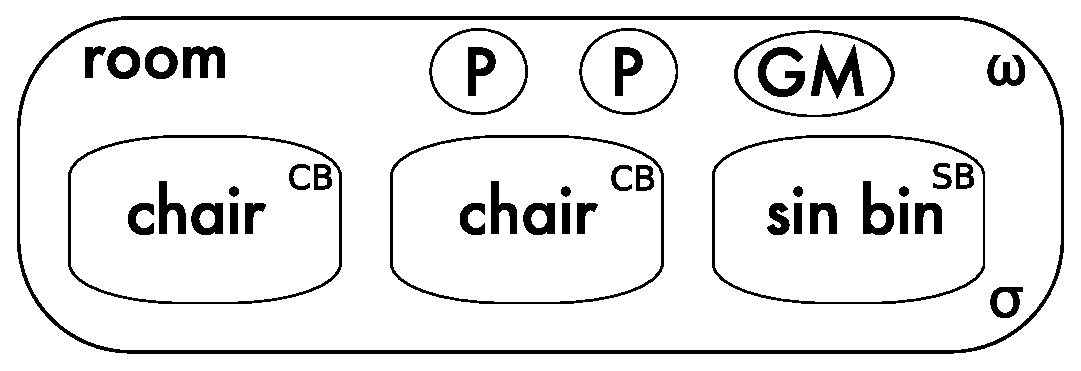
\includegraphics[scale=0.5]{gameenvbw}
  \caption{The Musical Chairs Environment}
  \label{fig:gameenv}
\end{figure}

The locality structure is represented graphically by Fig. \ref{fig:gameenv}
and in the calculus by the equation shown below.

\begin{equation}
\loc{room}{\nloc{chair}{\nil}{CB} \pc \nloc{chair}{\nil}{CB}
\pc \nloc{sin bin}{\nil}{SB} \pc P \pc P \pc GM}{\Omega}{\sigma}
\end{equation}

\noindent where $\nloc{m}{E}{F}$ is abbreviated from
$\loc{m}{E}{F}{\{\}}$.  The players themselves are represented by
\emph{processes}.  This allows them both to interact and to move between
localities.  A gamesmaster process is also introduced.  This doesn't
play an active role in the game itself, but is instead responsible for
performing the administrative duties of removing chairs from the game
and controlling player movement.  The process definitions are summarised
in Table \ref{tab:musicalchairs}, and make use of the derived syntax for
a clock prefix, $\sigma.P$, shown in \ref{clockcontrol}.

\begin{table}[h]
  \caption{Summary of Processes and Derived Syntax for Musical Chairs}
  \label{tab:musicalchairs}
  \shrule
  \begin{align}
   CB &
    \eqdef 
    \mu X.(\overline{in}.\overline{out}.X + \overline{open}.\Omega) \label{chairb} \\
   SB &
    \eqdef 
    \mu X.\overline{in}.X \label{sinb} \\
   GM1 &
    \eqdef 
    \sigma.GM2 \label{gmstage2} \\
    GM2 &
    \eqdef 
    open\ chair.GM3 \label{gmstage3} \\
   GM3 &
   \eqdef
   \sigma.GM4 \label{gmstage4} \\
   GM4 &
    \eqdef  
    \mu X.(\stimeout{\procin{sit}{chair}.X}{\sigma}{GM5}) \label{gmstage5} \\
   GM5 &
    \eqdef 
    \mu X.(\stimeout{\procin{leave}{sinbin}.X}{\sigma}{GM1}) \label{gmstage6}\\
    P &
    \eqdef 
    \sigma.\sigma.MP \label{player} \\
    MP &
    \eqdef
    \stimeout{sit.PIC}{\sigma}{L} \label{mplayer}\\
   PIC &
    \eqdef 
    \sigma.\sigma.PLC \label{pinchair} \\
   PLC &
   \eqdef
   \procout{stand}{chair}.0|stand.P \label{pleavechair} \\
   L &
    \eqdef 
    leave.0 \label{loser} 
  \end{align}
  \shrule
\end{table}

The presence of music is signified by the ticks of a clock, $\sigma$.  A
tick from $\sigma$ is also used to represent the implicit
acknowledgement that everyone who can obtain a chair has done so, and
that the remaining player left in the room has lost.  With regard to the
bouncers of the localities, the room locality is not prone to either
destruction or the entry or exit of other localities, having a bouncer
simply equal to $\Omega$.  This retains the encapsulation of the model
as a single room locality, and prevents other processes or localities
from interfering with its behaviour.

The definition of appropriate bouncers is essential for the chairs
(\ref{chairb}) and the sin bin (\ref{sinb}).  It is the chair bouncer
that enforces the implicit predicate that only one player may inhabit a
chair at any one time, while the sin bin bouncer prevents players
leaving the sin bin once they have entered.

To model stage one of the game, $n$ player processes and $n$ chair
locations are placed in the room.  The advantage of using TNT for this
model is that the actual number of players or chairs is irrelevant.
They only have to be equal at the start to accurately model the game.
The calculus allows the creation of a compositional semantics, as
discussed in chapter \ref{introduction}, which works with any $n$.

For the purposes of demonstration, $n$ is assumed to be two to give the
following starting state:

\begin{equation}
  \loc{room}{\nloc{chair}{\nil}{CB} \pc \nloc{chair}{\nil}{CB} \pc 
   Pr \pc P \pc GM1}{\Omega}{\sigma}.
\end{equation}

\noindent The room and chairs appear as shown earlier.  The player
processes (\ref{player}) simply wait until two clock
cycles have passed, the end of each being signalled by a tick from
$\sigma$.  The intermittent period between the ticks (the second clock
cycle) represents the playing of the music.  

Stage two, where the music is started, is thus represented simply by the
first tick of $\sigma$,

\begin{equation}
\begin{aligned}
  & \loc{room}{\nloc{chair}{\nil}{CB} \pc \nloc{chair}{\nil}{CB} \pc 
   P \pc P \pc
   GM1}{\Omega}{\sigma} \\
 \lderives{\sigma}\ & \loc{room}{\nloc{chair}{\nil}{CB} \pc \nloc{chair}{\nil}{CB} \pc 
   \sigma.MP \pc \sigma.MP \pc
   GM2}{\Omega}{\sigma}
\end{aligned}
\end{equation}

\noindent which the gamesmaster ($GM1$ (\ref{gmstage2})) also waits for,
before evolving into $GM2$ (\ref{gmstage3}).  The second cycle, prior
to the music stopping, is used to remove a chair from the game.  Maximal
progress, as explained in section \ref{introduction}, ensures that this
occurs before the next clock tick, as the removal emits a silent action.
The transition from stage three to stage four is thus as follows:

\begin{equation}
\begin{aligned}
& \loc{room}{\nloc{chair}{\nil}{CB} \pc \nloc{chair}{\nil}{CB} \pc 
   \sigma.MP \pc \sigma.MP \pc
   GM2}{\Omega}{\sigma} \\
 \lderives{\tau}\ & \loc{room}{\nil \pc \nloc{chair}{\nil}{CB} \pc 
   \sigma.MP \pc \sigma.MP \pc
   GM3}{\Omega}{\sigma}
\end{aligned}
\end{equation}

\noindent with one of the two chairs being chosen non-deterministically.
The second tick then occurs, leading in to stage five and the most
interesting part of the model.

\begin{equation}
\begin{aligned}
& \loc{room}{\nil \pc \nloc{chair}{\nil}{CB} \pc 
   \sigma.MP \pc \sigma.MP \pc
   GM3}{\Omega}{\sigma} \\
\lderives{\sigma}\ & \loc{room}{\nil \pc \nloc{chair}{\nil}{CB} \pc 
   MP \pc MP \pc
   GM4}{\Omega}{\sigma} \\
\end{aligned}
\end{equation}

The aim of stage five is to get as many player processes as possible
inside chair localities.  This is handled by again relying on maximal
progress to essentially perform a form of broadcast that centres on
mobile actions, as briefly mentioned in \ref{procmob}.  Rather than
sending a signal to a number of recipients, a request to move into a
chair (see (\ref{gmstage5}) and (\ref{mplayer})) is delivered instead.

If a chair is available, then a player process will enter it (the actual
chair and player chosen is non-deterministic).  This will cause an
internal action to occur, which takes precedence over the clock tick.
Thus, when the clock eventually does tick, it is clear that no more
players can enter chairs. Using clocks in this manner makes the system
\emph{compositional}; in contrast to other models, players and chairs
can be added without requiring changes to the process definitions.  In
this running example, there are two players, but only one chair, which
results in a single $\tau$ transition:

\begin{equation}
\begin{aligned}
& \loc{room}{\nil \pc \nloc{chair}{\nil}{CB} \pc 
   MP \pc MP \pc
   GM4}{\Omega}{\sigma} \\
\lderives{\tau}\ & \loc{room}{\nil \pc \nloc{chair}{\nil \pc PIC}{\overline{out}.CB} \pc 
   MP \pc
   GM4}{\Omega}{\sigma} \\
\end{aligned}
\end{equation}

\noindent that causes one of the $MP$ processes to move in to a
chair, and become a $PIC$ process.  This is followed by the
$\sigma$ transition, which marks the move to stage six.

\begin{equation}
\begin{aligned}
&  \loc{room}{\nil \pc \nloc{chair}{\nil \pc PIC}{\overline{out}.CB} \pc 
   MP \pc
   GM4}{\Omega}{\sigma} \\
\lderives{\sigma}\ & \loc{room}{\nil \pc \nloc{chair}{\nil \pc \sigma.PLC}{\overline{out}.CB} \pc 
   L \pc
   GM5}{\Omega}{\sigma} \\
\end{aligned}
\end{equation}

Both stage six and seven proceed in a similar way.  Stage six sees
essentially the same broadcasting behaviour applied to the losing
players (see (\ref{gmstage6}) and (\ref{loser})).  The difference is
that stage six demonstrates something which wouldn't be possible without
mobility: the broadcast is limited to those player processes which
remain in the room.  As communication between processes in different
localities is disallowed in TNT, an implicit scoping of the broadcast
occurs.  In the example, stage six again sees just one $\tau$
transition:

\begin{equation}
\begin{aligned}
&  \loc{room}{\nil \pc \nloc{chair}{\nil \pc \sigma.PLC}{\overline{out}.CB} \pc 
   L \pc
   GM5}{\Omega}{\sigma} \\
\lderives{\tau}\ & \loc{room}{\nil \pc \nloc{chair}{\nil \pc \sigma.PLC}{\overline{out}.CB} \pc
   GM5}{\Omega}{\sigma} \\
\end{aligned}
\end{equation}

\noindent which results in the remaining $MP$ (now a losing
process, $L$) moving to the sin bin.  Due to space constraints, the sin bin
locality is not shown in the above derivations.  It may be factored in
to the above as follows:

\begin{equation}
\begin{aligned}
& \nloc{sinbin}{\nil}{SB} \pc L \pc GM5 \\
\lderives{\tau} & \nloc{sinbin}{\nil \pc \nil}{SB} \pc GM5
\end{aligned}
\end{equation}

\noindent where the $L$ process evolves to become a simple $\nil$
process.  The broadcast is again terminated by a tick from $\sigma$,

\begin{equation}
\begin{aligned}
&  \loc{room}{\nil \pc \nloc{chair}{\nil \pc \sigma.PLC}{\overline{out}.CB} \pc
   GM5}{\Omega}{\sigma} \\
\lderives{\sigma}\ & \loc{room}{\nil \pc \nloc{chair}{\nil \pc PLC}{\overline{out}.CB} \pc
   GM1}{\Omega}{\sigma} 
\end{aligned}
\end{equation}

\noindent which, in this case, also signifies the music starting up again.  The
remaining players leave their chairs:

\begin{equation}
\begin{aligned}
& \loc{room}{\nil \pc \nloc{chair}{\nil \pc PLC}{\overline{out}.CB} \pc
   GM1}{\Omega}{\sigma}   \\
\lderives{\tau}\ & \loc{room}{\nil \pc \nloc{chair}{\nil \pc \nil}{CB} \pc
   GM1 \pc P}{\Omega}{\sigma} 
\end{aligned}
\end{equation}

\noindent and the system essentially returns to the beginning, with $n -
1$ chairs and $n - 1$ players.

\section{The Type System}
\label{typesys}

This final section focuses on the specification of a simple type
system for the calculus, which fulfills two goals:

\begin{enumerate}
\item Ensures the sanity of a given TNT construction, which is
  implicit in the examples above.  This is primarily achieved by
  ensuring that normal process primitives and the primitives used by
  bouncers remain distinct.  For example,
  $\ambin{n}.\overline{in}.\nil$ should not be a valid bouncer,
  especially as $\ambin{n}$ suggests that the bouncer (and its locality)
  should move inside $n$.
\item Restrict mobility by type in addition to cardinality.  With the
  syntax and semantics alone, movement control is limited to how many
  times a locality may entered or exited.  With the addition of a type
  system, these operations can be restricted to processes whose type
  allows the action to take place.
\end{enumerate}

The concepts behind this are based on the type systems presented for
the ambient calculus (see \ref{ambienttypes}), specifically the
notion of groups presented in \cite{ambienttypes} and \cite{m3}.

Each process is a member of a group, which determines the use of the
mobility primitives.  Each group has a type\footnote{Or, more
  accurately, as groups are types themselves, it essentially has a
  type of a type or a \emph{kind}} composed of the following sets of
locality names:

\begin{itemize}
\item $\mathscr{R}$ -- Localities which may be \emph{resided} in
\item $\mathscr{O}$ -- Localities which may be \emph{opened}
\item $\mathscr{L}$ -- Localities which may be \emph{left}
\item $\mathscr{E}$ -- Localities which may be \emph{entered}
\end{itemize}

$\mathscr{L}$ and $\mathscr{E}$ form subsets of $\mathscr{R}$, as
clearly, if a process may enter or leave a locality, it must also be
able to reside within it.  As an example, consider the group
$(\{n\},\emptyset, \emptyset,\{n\})$.  Processes which are members of
this group may enter and reside in $n$, but, once in $n$, they may not
leave.  They also lack the ability to destroy $n$.

Table \ref{tab:basictypes} presents the basic rules and the rudimentary
types used for the basic parts of the syntax, such as $\nil$.  As is
standard in the literature, the types are defined with respect to a type
environment, $\Gamma$.  On this note, the rule $Env$ simply states that
if $\xi$ of type $T$ is a member of $\Gamma$, then a typing derivation
$\vdash \xi : T$ may be made in the context of $\Gamma$.  This forms the
basis of all later rules.

\begin{table}
  \caption{Types: Basics}
  \label{tab:basictypes}
  \shrule
 \begin{center}
 \begin{tabular}{rc}
     \Rule{Env}
     {\xi : T \in \Gamma}
     {\Gamma \vdash \xi : T}
     {}
  &
  \Rule{Nil}
     {\Gamma \vdash g : Group}
     {\Gamma \vdash \nil : g}
     {}
  \\[3ex]
     \Rule{BNil}
     {-}
     {\Gamma \vdash \Omega : Bouncer}
     {}
     &
     \Rule{Stop}
     {\Gamma \vdash g : Group}
     {\Gamma \vdash \Delta : g}
     {}
     \\[3ex]
     \Rule{Stall}
     {\Gamma \vdash \sigma : Clock, g : Group}
     {\Gamma \vdash \Delta_\sigma : g}
     {}
     &
     \Rule{Act}
     {\Gamma \vdash \alpha : Lab, P : g : Group}
     {\Gamma \vdash \alpha . P : g}
     {}
  \\[3ex]
     \Rule{Rec}
     {\Gamma \vdash P : g : Group}
     {\Gamma \vdash \mu X.P : g}
     {}
     &
     \Rule{Res}
     {\Gamma \vdash a : Act, P : g : Group}
     {\Gamma \vdash P \setminus a : g}
     {}
 \end{tabular}
  \end{center}
  \shrule
\end{table}

The remaining rules in Table \ref {tab:basictypes} provide types for
the processes.  Via $Nil$ and $Stop$, both $\nil$ and $\Delta$ are
given a type of $g$, where $g$ is a group.  The only precondition for
these derivations is that $g$ is typeable as a $Group$ in the
environment, $Gamma$.  Likewise, $\Omega$ can be typed as a $Bouncer$,
thus distinguishing it from the normal processes, such as $\nil$.

The other rules are also relatively simple.  $Stall$ simply says that
$\Delta_{\sigma}$ may be typed as a process of group $g$ if $\sigma$
is a clock.  $Act$ states that $\alpha.P$ is a process in $g$ if
$\alpha$ is typeable as a label ($Lab$, which includes actions,
co-actions and $\tau$) and $P$ is also typeable as a process in the
same group.  In the same vein, $Rec$ and $Res$ type recursive and
restricted processes respectively, if the constituent process, $P$, is
already typeable as a process.  In the case of $Res$, $a$ must be an
action ($Act$) if the process is to be successfully typed.

In Table \ref{tab:operatortypes}, types are given to the composition of
processes using the binary operators for summation, parallel composition
and timeout.  All four are mostly identical, providing a type for the
process resulting from the combination of the operator with two other
processes, $P$ and $P^\prime$.  Each process is given a type, which must
be equivalent groups within the union of the two environments, $\Gamma$
and $\Gamma^\prime$.

\begin{table}
  \caption{Types: Operators}
  \label{tab:operatortypes}
  \shrule
 \begin{center}
 \begin{tabular}{c}
     \Rule{Sum}
     {\Gamma \vdash P : g,
      \Gamma^\prime \vdash P^\prime : g^\prime,
      \Gamma \cup \Gamma^\prime \vdash g = g^\prime : Group}
     {\Gamma \cup \Gamma^prime \vdash P + P^\prime : g}
     {}
     \\[3ex]
     \Rule{Par}
     {\Gamma \vdash P : g,
      \Gamma^\prime \vdash P^\prime : g^\prime,
      \Gamma \cup \Gamma^\prime \vdash g = g^\prime : Group}
     {\Gamma \cup \Gamma^prime \vdash P \mid P^\prime : g}
     {}
     \\[3ex]
     \Rule{FTO}
     {\Gamma \vdash P : g,
      \Gamma^\prime \vdash P^\prime : g^\prime,
      \Gamma \cup \Gamma^\prime \vdash \sigma : Clock,
      \Gamma \cup \Gamma^\prime \vdash g = g^\prime : Group}
     {\Gamma \cup \Gamma^\prime \vdash \timeout{P}{\sigma}{P^\prime} : g}
     {}
  \\[3ex]
  \Rule{STO}
     {\Gamma \vdash P : g,
      \Gamma^\prime \vdash P^\prime : g^\prime,
      \Gamma \cup \Gamma^\prime \vdash \sigma : Clock,
      \Gamma \cup \Gamma^\prime \vdash g = g^\prime : Group}
     {\Gamma \cup \Gamma^\prime \vdash \stimeout{P}{\sigma}{P^\prime} : g}
     {}
     \\[3ex]
     \Rule{BSum}
     {\Gamma \cup \Gamma^\prime \vdash B : Bouncer,
      \Gamma \cup \Gamma^\prime  \vdash B^\prime : Bouncer}
     {\Gamma \cup \Gamma^\prime \vdash B + B^\prime : Bouncer}
     {}
 \end{tabular}
  \end{center}
  \shrule
\end{table}

The only other issue worthy of note with respect to these rules is that
$FTO$ and $STO$ also require that $\sigma$ is typeable as a clock,
another restriction which simply makes explicit a number of issues
implied in the syntax.  Table \ref{tab:operatortypes} also includes
a summation rule for bouncers, which simply requires that each bouncer
is typeable as a $Bouncer$ under the union of the two type environments,
$\Gamma$ and $\Gamma^\prime$.

The types in Tables \ref{tab:basictypes} and \ref{tab:operatortypes}
provide the basis for the mobility types presented in Table
\ref{tab:mobilitytypes}, which form the focus of this type system.
$g(\mathscr{R})$, $g(\mathscr{O})$, $g(\mathscr{L})$ and
$g(\mathscr{E})$ represent the sets of locality names that form the
group, $g$.

\begin{table}
  \caption{Types: Mobility}
  \label{tab:mobilitytypes}
  \shrule
 \begin{center}
 \begin{tabular}{c}
     \Rule{Loc}
     {\Gamma \vdash m : Locality,
     \Gamma \vdash P : g : Group,
     \Gamma \vdash B : Bouncer,
     m \in g(\mathscr{R})}
     {\Gamma \vdash \loc{m}{P}{B}{\vec{\sigma}} : g}
     {}
  \\[3ex]
     \Rule{LocIn}
     {\Gamma \vdash m : Locality,
  \Gamma \vdash P : g : Group,
  m \in g(\mathscr{E})}
     {\Gamma \vdash \ambin{m}.P : g}
     {}
     \\[3ex]
     \Rule{LocOut\ \ }
     {\Gamma \vdash \loc{n}{\loc{m}{P}{B_1}{\vec{\sigma}}}{B_2}{\vec{\rho}} : g : Group,
  m \in g(\mathscr{L}),
  n \in g(\mathscr{E})}
     {\Gamma \vdash \ambout{m}.P : g}
     {}
     \\[3ex]
     \Rule{Open}
     {\Gamma \vdash \loc{n}{P}{B_1}{\vec{\sigma}} : g : Group,
  \Gamma \vdash \loc{m}{Q}{B}{\vec{\sigma}} : h : Group,
  m \in g(\mathscr{O}),
  n \in h(\mathscr{E})}
     {\Gamma \vdash \ambopen{m}.P : g}
     {}
  \\[3ex]
     \Rule{AmbIn\ \ }
  {\Gamma \vdash a : Act,
  \Gamma \vdash \loc{n}{P \mid Q \mid \loc{n}{\nil}{B_1}{\vec{\sigma}}}{B_2}{\vec{\rho}} : g : Group, 
  m \in g(\mathscr{E})}
     {\loc{n}{\procin{a}{m}.P \mid a.Q \mid \loc{n}{\nil}{B_1}{\vec{\sigma}}}{B_2}{\vec{\rho}} : g : Group}
     {}  
  \\[3ex]
     \Rule{AmbOut\ \ \ \ }
  {\Gamma \vdash a : Act,
  \Gamma \vdash \loc{n}{\loc{m}{P \mid Q}{B_1}{\vec{\sigma}}}{B_2}{\vec{\rho}} : g : Group, 
  m \in g(\mathscr{L}),
  n \in g(\mathscr{E})}
     {\Gamma \vdash \loc{n}{\loc{m}{\procout{a}{m}.P \mid a.Q}{B}{\vec{\sigma}}}{B_2}{\vec{\rho}} :
  g}
     {}  
 \end{tabular}
  \end{center}
  \shrule
\end{table}

$Loc$ is a fundamental rule, which links localities, bouncers, clocks
and processes.  If $m$ is a locality name ($Locality$), $P$ is a process
of type $g$ (where $g$ is a $Group$) and $B$ is a $Bouncer$, then the
process $P$ may be typed as $g$ while encapsulated within the locality
$m$, with its bouncer $B$.  The later rules rely on this to provide a
type for the existing localities.

$LocIn$, $LocOut$ and $Open$ are fairly similar, all relating to whether
a particular location movement is typeable, based on the groups of the
processes within them.  $LocIn$ states that if $m$ is a locality name,
and $P$ is a process typed with the group, $g$, then $P$ may be prefixed
with the $\ambin{m}$ capability if m is an element of the set
$g(\mathscr{E})$, where $g(\mathscr{E})$ is the set of locality names which
members of group $g$ may enter.

The $LocOut$ rules differs from $LocIn$ in that it provides a context
for the movement which will occur when $\ambout{m}$ is performed.  This
is necessary because, not only must the resulting process,
$\ambout{m}.P$, be able to leave $m$, but it also must be able to enter
the locality above, $n$.  This is unnecessary in $LocIn$ as $P$ does not
leave the locality above.  These restrictions are enforced by requiring
that the group of $P$, $g$, has $m$ as an element of $g(\mathscr{L})$ (so
$P$ can leave $m$) and $n$ as an element of $g(\mathscr{E})$ (so $P$ can
enter $n$).

$LocOpen$ has similar requirements.  $P$ is the process that performs
the capability, $\ambopen{m}$, which requires its group, $g$, to contain
$m$ in the set of locality names which may be opened.  However, the
destruction of $m$ also has an effect on processes located in $m$,
represented as $Q$.  As a result, $Q$ must have an appropriate group,
$h$, such that $Q$ can reside in the parent locality, $n$, after $m$ is
opened.  $AmbIn$ and $AmbOut$ are nearly identical to $LocIn$ and
$LocOut$; the main difference is that they must provide additional
contextual information (as well as requiring the typeability of the
action, $a$) in order to handle the involvement of two processes rather
than simply one.

The final table, \ref{tab:bouncertypes}, adds some simple rules to
complete the typing of the bouncers.  $BRec$ allows recursive bouncers
to be defined, while $BIn$, $BOut$ and $BOpen$ allow an existing
bouncer, $B$, to be prefixed with one of the three co-capabilities
($\bin$, $\bout$ and $\bopen$).

\begin{table}
  \caption{Types: Bouncers}
  \label{tab:bouncertypes}
  \shrule
 \begin{center}
 \begin{tabular}{rc}
  \Rule{BRec}
  {\Gamma \vdash B : Bouncer}
  {\Gamma \vdash \mu X.B : Bouncer}
  {}
  &
  \Rule{BIn}
  {\Gamma \vdash B : Bouncer}
  {\Gamma \vdash \bin .B : Bouncer}
  {}
  \\[3ex]
  \Rule{BOut}
  {\Gamma \vdash B : Bouncer}
  {\Gamma \vdash \bout .B : Bouncer}
  {}
  &
  \Rule{BOpen\ }
  {\Gamma \vdash B : Bouncer}
  {\Gamma \vdash \bopen .B : Bouncer}
  {}
  \end{tabular}
  \end{center}
  \shrule
\end{table}
